\newpage
\subsection{Расчёт освещения} \label{lighting_calculation}

Произведем расчет системы освещения, так как этот физический фактор относится
к вредным и не удовлетворят поставленным требованиям. Возможность нормальной
производственной деятельности в научно~--~исследовательских организациях должна быть
обеспечена оптимально спроектированным и выполненным освещением. Сохранность зрения
работника, состояние его нервной системы, безопасность на производстве зависит от
условий освещения.

При освещении помещений используют \textit{естественное}, \textit{искусственное},
а также \textit{смешанное} освещение.
Естественное освещение подразделяют на \textit{боковое}, \textit{верхнее} и
\textit{комбинированное}.
Искусственное освещение по конструктивному исполнению делится на две системы:
\textit{общее} и \textit{комбинированное}. Применение одного местного освещения
внутри помещения не допускается.

Основная задача освещения – создание наилучших условий для зрения. Для ее
выполнения освещение должно отвечать следующим требованиям:

\begin{enumerate}
    \item   Освещенность на рабочем месте должна соответствовать характеру
            зрительной работы, которая определяется тремя параметрами
        \begin{itemize}
            \item объектом различия
            \item фоном с определенным коэффициентом отражения (0.02~--~0.95)
            \item контрастностью объекта
        \end{itemize}
    Контрастность определяется как:
    \begin{equation}
    \label{lighting_contrast}
        K = \frac{L_0 - L_\text{ф}}{L_\text{ф}}
    \end{equation}
    где $L_0$, $L_\text{ф}$ - яркость объекта и фона соответственно

    Средняя величина контрастности $0.2 - 0.3$. До определенного предела увеличения
    яркости повышает производительность труда.

    \item   Необходимо обеспечивать равномерную яркость на всей рабочей поверхности.
            В поле зрения не должны находиться предметы, резко отличающиеся по яркости.

    \item   По рабочей поверхности не должно быть резких теней и не должно быть
            блесткости, т.е. повышения яркости светящихся поверхностей.

    \item   Величина освещенности должна быть постоянной по времени, что достигается
            стабилизацией напряжения питания и сглаживанием пульсаций тока в
            осветительных приборах.

    \item   Выбирается оптимальный спектральный состав освещения путем комбинации
            естественного и искусственного освещений.

    \item   Все электроосветительные приборы должны быть электро~- и травмобезопасны.
\end{enumerate}

Основным видом работ, выполняемых инженером~--~разработчиком, является программирование
и черчение на ПЭВМ, расчетные работы с использованием микрокалькуляторов и вычислительной
техники. Величина минимальной освещенности устанавливается по характеру зрительной работы.

\subsubsection{Искусственное освещение помещения}

Определение необходимой мощности осветительной установки для получения заданной
освещенности требует решения следующих вопросов:

\begin{itemize}
    \item \textit{выбор типа источника света}: применение горизонтальных ламп с
    большей светоотдачей оправдано, т.к. в поле зрения инженера~--~разработчика
    нет быстровращающихся предметов и пульсации светового потока практически не
    заметны

    \item \textit{выбор системы освещения}: выбираем комбинированную систему
    согласно СНиП 23.05-95 \cite{ecology_snip_23_05_95}. Система общего освещения
    создает равномерное распределение света. Для повышения общего освещения
    используют местные светильники, обеспечивающие создание направленного света,
    исключающие отраженную блесткость, а также позволяющие выполнять просвечивание
    материалов и деталей

    \item \textit{выбор типа светильников}: исходя из требований, предъявляемых
    к светильникам, выбираем тип светильника – ЛОУ (люминесцентные светильники
    расположенные в светящую линию), устанавливаемый в помещениях с небольшой
    запыленностью и нормальной влажностью

    \item \textit{распределение светильников в помещении и их количество}:
    равномерность распределения освещенности светильниками ЛОУ достигается в случае,
    если расстояние между центрами светильников больше высоты их расположения над
    рабочей поверхностью $H_p$ в 1.4 раза
\end{itemize}

Примем следующие параметры:
\begin{table}[h!]
    \centering
    \begin{tabular}{l|l}
        \hline
        Освещенность комбинированная    & $E_\text{комб.общ}$ = 400 лк  \\
        Освещенность общая              & $E_\text{общ}$ = 150 лк       \\
        Коэффициент запаса              & k = 1.3                       \\
        \hline
    \end{tabular}
    \caption{Общие параметры искуственного освещения}
    \label{artificial_lighting_parameters}
\end{table}

\subsubsection{Общее освещение помещения}

\begin{table}[ht]
    \centering
    \begin{tabu}{X[l,m]|X[l,m]}
        \hline
        Высота помещения                                                        & $H$ = 3.2 м                                   \\
        Расстояние светильников от перекрытия                                   & $h_c$ = 0.25 м                                \\
        Высота светильников над полом                                           & $h_\text{п} = H - h_c$ = 2.95 м               \\
        Высота расчетной поверхности                                            & $h_p$ = 0.7 м                                 \\
        Расчетная высота                                                        & $h = h_\text{п} - h_p$ = 2.25 м               \\
        Расстояние между соседними светильниками по длине помещения             & $L_\text{д}$ = 3.2 м                          \\
        Расстояние между соседними светильниками по ширине помещения            & $L_\text{ш}$ = 3 м                            \\
        Расстояние от крайних светильников до стены                             & $l_\text{д} = 0.3 \cdot L_\text{д}$ = 0.96 м, \newline
                                                                                  $l_\text{ш} = 0.3 \cdot L_\text{ш}$ = 0.73 м  \\
        \hline
    \end{tabu}
    \caption{Параметры размещения светильников}
    \label{lamps_arrangement_parameters}
\end{table}

Используем метод коэффициента использования светового потока, предназначенный для
расчета общего равномерного освещения горизонтальных поверхностей при отсутствии
крупных затемняющих предметов.

Необходимый поток ламп в каждом светильнике:
\begin{equation}
\label{one_lamp_stream}
    \text{Ф} = \frac{E \cdot S \cdot k_\text{зап} \cdot k_\text{неравн}}{N \cdot k_\text{исп}}
\end{equation}
где $E$ = 300 лк - заданная минимальная освещенность для 3-го разряда зрительных работ, \\
$k_\text{зап}$ = 1.3 - коэффициент запаса для помещений, связанных с работой на ПЭВМ,   \\
$S = 40 ~\text{м}^2$ - освещаемая площадь,                                              \\
$N$ - намечаемое число светильников,                                                    \\
$k_\text{исп}$ – коэффициент использования,                                             \\
$k_\text{неравн}$ = 1.1 – коэффициент неравномерности освещения для данных $l_\text{ш}$ и
$l_\text{д}$

Для нахождения коэффициента использования $k_\text{исп}$ по справочным таблицам
выберем индекс помещения $i = 1.5$ для ранее вычисленной расчётной высоты $h$ и
примерно оценим коэффициенты отражения поверхностей помещения:
\begin{equation}
    \begin{array}{ll}
        r_\text{потолок}    & = 70\% \\
        r_\text{стены}      & = 50\% \\
        r_\text{пол}        & = 30\% \\
    \end{array}
    \label{reflection_coeff}
\end{equation}

Тогда из справочных таблиц для освещаемой площади $S$ получим коэффициент использования
$$
    k_\text{исп} = 0.59
$$

Светильники с люминесцентными лампами в помещениях для работы рекомендуют
устанавливать рядами. Положим $N = 4$ как 2 светильника в два ряда.

Подставив вышеописанные параметры в формулу (\ref{one_lamp_stream}), получим
необходимый световой поток одного светильника

$$
    \text{Ф} \simeq 7200 ~\text{лм}
$$

Исходя из этого, используем светильники с люменесцентными лампами 2х40 Вт с
общим потоком 7200 лм.

Параметры светильника типа ЛОУ:

\begin{tabular}{ll}
    - мощность    & 2x40 Вт   \\
    - длина       & 1.44 м    \\
    - ширина      & 0.27 м    \\
    - высота      & 0.10 м    \\
\end{tabular}

Схема расположения светильников показана на рис. (\ref{pic_lamps_arrangement}).

\begin{figure}[ht]
    \centering
    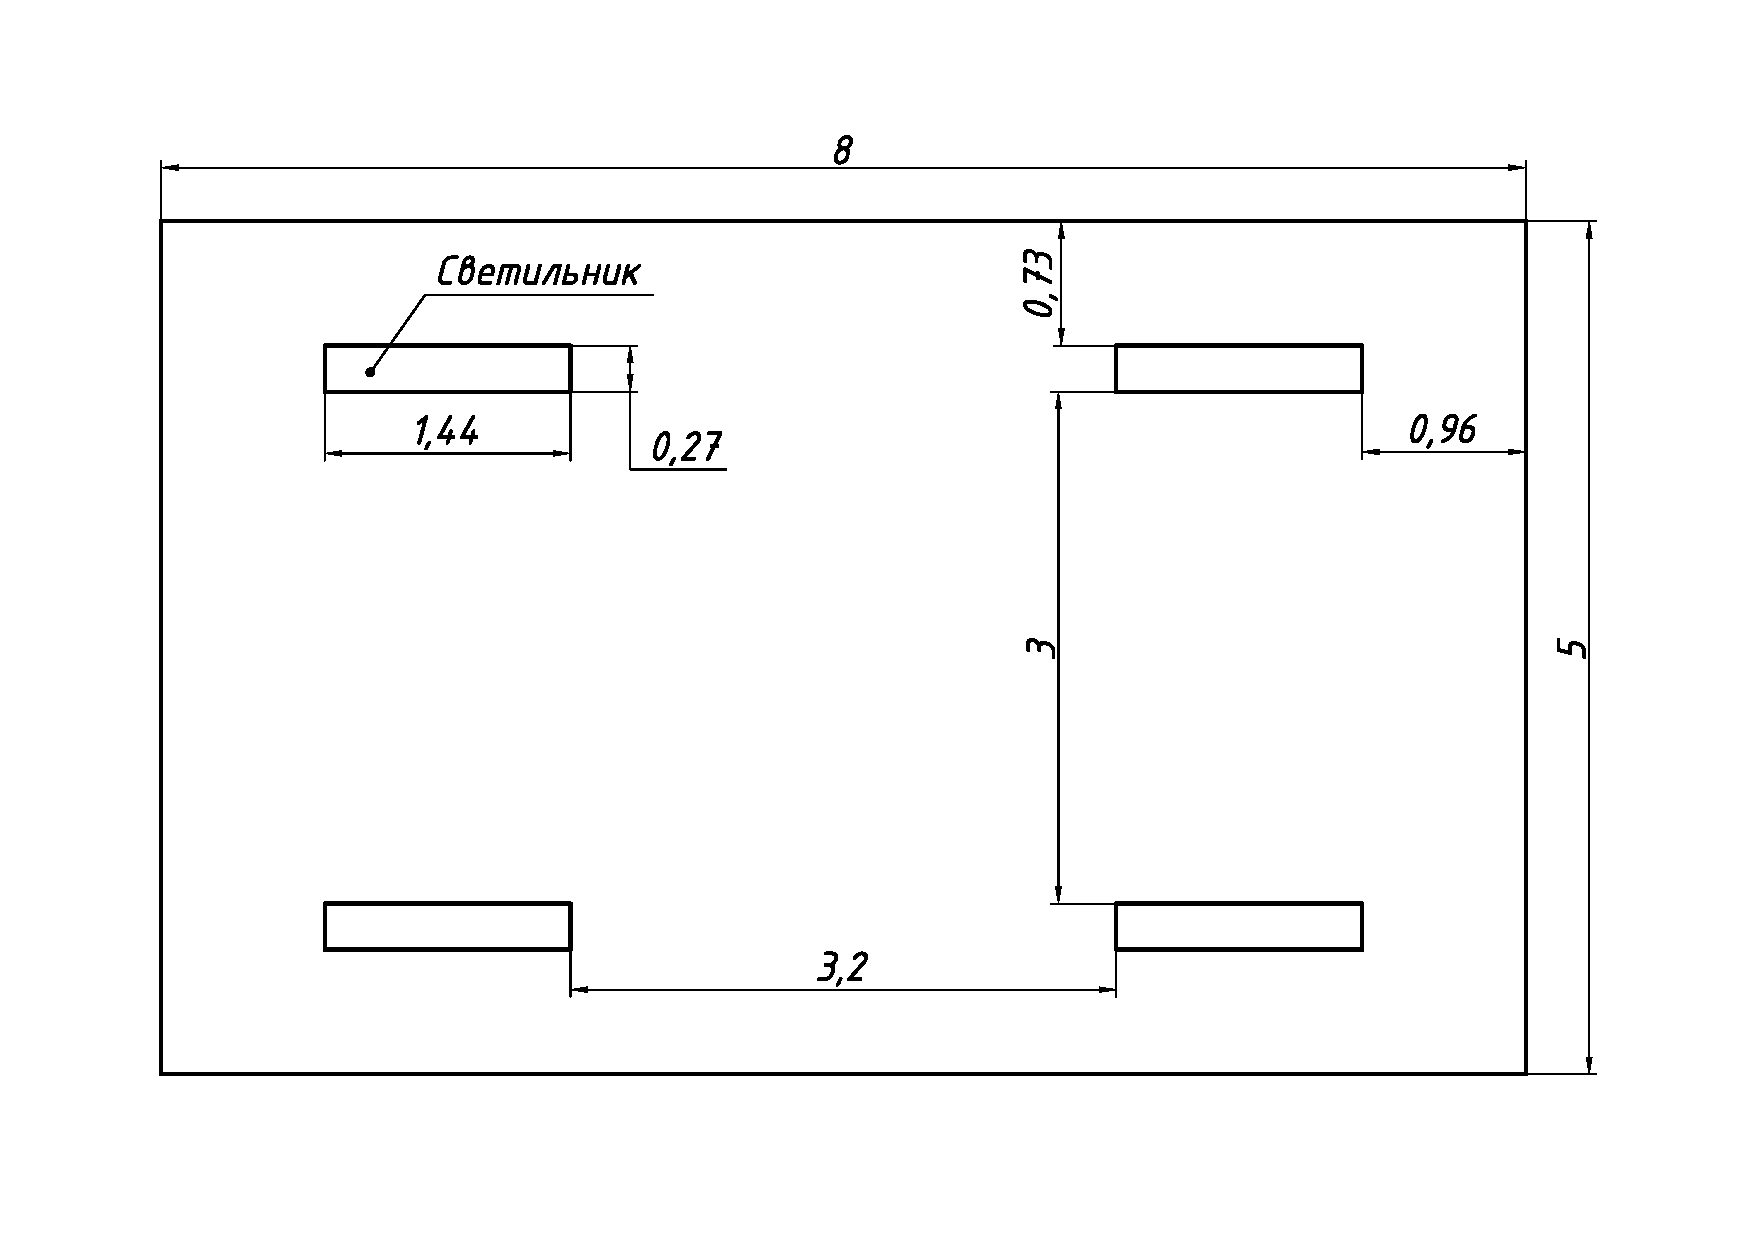
\includegraphics[width=\textwidth, keepaspectratio, clip=true, trim=0mm 25mm 0mm 20mm]
                    {./src/ecology/pictures/lights_arrangement}
    \caption{Схема расположения светильников (размеры в метрах)}
    \label{pic_lamps_arrangement}
\end{figure}


\subsubsection{Комбинированное освещение помещения}

Система комбинированного освещения заключается в дополнительной установке
светильников местного освещения, предназначенных для освещения зоны расположения
документов.

Сила света источника в направлении точки А определяется по следующей формуле:

\begin{equation}
    Y_A = \frac{E \cdot h^2}{\cos \alpha}
    \label{light_source_power_in_dot_direction}
\end{equation}
где $E$ - освещённость от местного источника света                      \\
$h$ - расчетная высота из таблицы (\ref{lamps_arrangement_parameters})  \\
$\alpha$ -  угол падения лучей света относительно нормали к поверхности

\begin{equation}
    E = E_\text{комб.общ} - E_\text{комб.общ}
    \label{combined_lighting_illumination}
\end{equation}

Подставив в формулу (\ref{combined_lighting_illumination}) значения из таблицы
(\ref{artificial_lighting_parameters}), получим

$$
    E = 250 ~\text{лк}
$$

При $\alpha = 45 \degree$ сила света будет равна

$$
    Y_A = 1790 ~\text{Кд}
$$

В местных светильниках будем использовать лампы накаливания вакуумные HB 220-100
с силой света $Y_\text{ламп} = 1425$ Кд. Тогда в одном светильнке должно быть следующее число
ламп

$$
    n_\text{ламп} = \frac{Y_A}{Y_\text{ламп}} = 1.26 \simeq 2
$$

\subsubsection{Естественное освещение помещения}

Цель данного расчета - убедиться, что площадь остекления на рабочем месте
инженера~--~разработчика обеспечивает величину нормированного коэффициента
естественной освещенности.

В рабочем месте имеет место боковое ествественное освещение (через окна).

Необходимая площадь световых проёмах определяется в соответствии с
\cite{lighting_calc_method}[ф-ла 2.3] как

\begin{equation}
    S_o = \frac{S_n \cdot e_N \cdot k_\text{з} \cdot \eta_o}{100 \cdot \tau_\text{общ} \cdot r_1}
            \cdot k_\text{зд}
    \label{windows_area}
\end{equation}
где $S_n$ - площадь пола помещения, $\text{м}^2$,                                   \\
$e_N$ - нормированное значение коэффициента естественной освещенности для зданий,
расположенных в различных районах,                                                  \\
$k_\text{з}$ - коэффициент запаса,                                                  \\
$\eta_o$ - световая характеристика окна,
$\tau_\text{общ}$ - общий коэффициент светопропускания,                             \\
$r_1$ - коэффициент, учитывающий повышение КЕО при боковом освещении, благодаря
свету, отраженному от поверхностей помещения и подстилающего слоя, прилегающего
к зданию                                                                            \\
$k_\text{зд}$ - коэффициент, учитывающий затенение окон противостоящими зданиями

Нормированное значение коэффициента естественной освещенности для данного
района расположения определяется в соответствии с \cite{ecology_snip_23_05_95}[ф-ла 1]
по формуле

\begin{equation}
    e_N = e_\text{н} \cdot m_N
    \label{natural_lighting_koeff}
\end{equation}
где $e_\text{н}$ - ненормированный коэффициент естественной освещенности, \\
$m_N$ - коэффициент светового климата

Из \cite{ecology_snip_23_05_95}[табл. 1] для зрительной работы средней точности
(3-й разряд зрительной работы) получим
$$
    e_\text{н} = 1.5
$$

Так как по \cite{ecology_snip_23_05_95}[прилож. Д] Московский административный
район соответсвует 1-й группе по ресурсам светового климата и окна рабочего
помещения выходят на северо-восток, то по \cite{ecology_snip_23_05_95}[табл. 4]
$$
    m_N = 1
$$

Подставив эти значения в формулу (\ref{natural_lighting_koeff}), получим
$$
    e_N = 1.5
$$

Коэффициент запаса для общественных зданий, содержащих малое количество пыли
(менее 1 ~$\text{мг/м}^3$) равен
$$
    k_\text{з} = 1
$$

Найдем световую характеристику световых проемов по
\cite{lighting_calc_method}[табл. 2.3] при отношении длины помещения к его глубине
равном $0.625 \simeq 1$ в соответствии с геометрией помещения рис. (\ref{pic_lamps_arrangement})
и отношении глубины помещения к высоте от рабочей поверхности до верха окна,
соответствующей расчётной высоте из таблицы (\ref{lamps_arrangement_parameters}),
равном $3.56 \simeq 4$
$$
    \eta_o = 21
$$

Определяем общий коэффициент светопропускания по формуле
\cite{lighting_calc_method}[ф-ла 2.5]
\begin{equation}
    \tau_\text{общ} = \tau_1 \cdot \tau_2 \cdot \tau_3 \cdot \tau_4
    \label{overall_light_pass_koeff}
\end{equation}
где $\tau_1$ - коэффициент светопропускания материала,                          \\
$\tau_2$ - коэффициент, учитывающий потери света в переплетах светопроема,      \\
$\tau_3$ - коэффициент, учитывающий потери света в несущих конструкциях,        \\
$\tau_4$ - коэффициент, учитывающий потери света в солнцезащитных устройствах

$\tau_1 = 0.8$ для двойного листового оконного стекла в соответствии с
\cite{lighting_calc_method}[табл. 2.5].

$\tau_2 = 0.75$ для одинарного открывающегося оконного переплёта в соответствии с
\cite{lighting_calc_method}[табл. 2.6].

$\tau_3 = 1$ при боков естественном освещении, $\tau_4 = 1$ для убирающихся
регулируемых штор  в соответстии \cite{lighting_calc_method}[стр. 8].

Подставив эти значения в формулу (\ref{overall_light_pass_koeff}), получим
$$
    \tau_\text{общ} = 0.6
$$

Для определения $r_1$ необходимо определить величину средневзвешенного коэффициента
отражения $\rho_\text{ср}$ потолка, стен и пола по формуле
\cite{lighting_calc_method}[ф-ла 2.6]

\begin{equation}
    \rho_\text{ср} = \frac{ r_\text{пол} \cdot S_\text{пол}
                            + r_\text{потолок} \cdot S_\text{потолок}
                            r_\text{стены} \cdot S_\text{стены}}
                            {S_\text{пол} + S_\text{потолок} + S_\text{стены}}
    \label{average_reflection_coeff}
\end{equation}

Из геометрии помещения
\begin{equation}
    \begin{array}{ll}
        S_\text{потолок}    & = 40 ~\text{м}^2      \\
        S_\text{стены}      & = 83.2 ~\text{м}^2    \\
        S_\text{пол}        & = 40 ~\text{м}^2      \\
    \end{array}
    \label{work_room_areas}
\end{equation}

Подставляя в формулу (\ref{average_reflection_coeff}) величины из (\ref{reflection_coeff})
и (\ref{work_room_areas}), получим
$$
    \rho_\text{ср} = 50 \%
$$

В соответствии с ранее найденными соотношениями геометрических параметров помещения,
получим из \cite{lighting_calc_method}[табл. 2.12]
$$
    r_1 = 7.3
$$

Так как окна производственного помещения не затенены соседними зданиями, то
$$
    k_\text{зд} = 1
$$

Подставив все полученные величины в формулу (\ref{windows_area}), получим
минимально необходимую площадь световых проёмов
$$
    S_o = 3.9 \text{ м}^2
$$

Полученная величина меньше реальной площади световых проёмов рабочего
помещения, значит требования СНиП 23.05-95 \cite{ecology_snip_23_05_95} выполнены.

\subsubsection{Контроль освещения}

Для создания рациональных условий и обеспечения необходимой освещенности, экономии
электроэнергии обеспечивается повседневный уход за установками освещения. Основные
мероприятия заключаются в следующем:

\begin{enumerate}
    \item   Контроль правильности подключения ламп (мигание), а также пускорегулирующих
            устройств (шум дросселей)
    \item   Очищение стекол световых проемов 2-4 раза в год в зависимости от запыленности,
            очистка светильников (4-12 раз в год) по мере загрязнения
    \item   Замена ламп (перегоревших или групп по мере выработки ресурса)
    \item   Проверка уровня освещенности после замены ламп
\end{enumerate}

\subsubsection{Выводы}

Произведен обоснованный выбор систем искусственного освещения, местного освещения,
а так же показано, что условия естественного освещения соответствуют принятым нормам.

На основании проведенных расчётов, освещение в рабочем помещении можно отнести
к оптимальному классу условий труда.
